
% -------- VARIABLES -------------------------------------------------------
\newcommand{\lectureVar}{Rechnersysteme \& -Netze}
\newcommand{\moduleVar}{Systeme 1}
\newcommand{\semesterVar}{WiSe 20/21}
\newcommand{\authorVar}{Noah Kamara}



% -------- PACKAGES --------------------------------------------------------
% Document Class
\documentclass[12pt]{report}

% Page Layout & Formatting
\usepackage[a4paper,width=150mm,top=25mm,bottom=25mm]{geometry} % Layout
\usepackage{fancyhdr} % Headers
\usepackage{titlesec} % Titles
\usepackage[many]{tcolorbox} % Boxes (Definitions, Examples)
\usepackage{graphicx} % Images / Other Graphics
\usepackage{float} % Floats (like Minipage) alignment
\usepackage{parskip} % no indents in new par

% Language Specific
\usepackage[utf8]{inputenc}
\usepackage[german]{babel} 

% Tables & Arrays
\usepackage{array}   % column types / tables
\usepackage{multicol} % tables, multicolumn

\usepackage{caption} % Caption styling
\usepackage{xcolor}



% -------- HEADERS, FOOTERS & TITLES ---------------------------------------
\pagestyle{fancy}
\fancyhf{}

\renewcommand{\chaptermark}[1]{\markboth{#1}{}}
\renewcommand{\headrulewidth}{1pt}
\renewcommand{\footrulewidth}{1pt}

% Header
\setlength{\headheight}{30pt}
\lhead{\moduleVar\\\lectureVar}
\rhead{\semesterVar\\\authorVar}

% Footer
\cfoot{\thepage}

% Titles
\titleformat{\section}[display]{\normalfont\bfseries}{}{0pt}{\Huge}



% -------- MATH MODE -------------------------------------------------------
% Math Mode Table Columns
\newcolumntype{L}{>{$}l<{$}}
% Überträge
\def\cred{\hbox to0pt{\textcolor{blue}{${}_{\tt 1}$}\hss}}



% -------- COLORS ----------------------------------------------------------
% Text Colors
\definecolor{mainColor}{HTML}{121113}
\definecolor{secColor}{HTML}{222725}

% ColorBox Colors
\definecolor{defboxColor}{HTML}{B5D99C}
\definecolor{infoboxColor}{HTML}{FFFF82}
\definecolor{boxbgColor}{HTML}{F2F2F2}



% -------- Color Boxes ----------------------------------------------------- 
% Definition Box
\newtcolorbox{defbox}[1][]{
	title=\textbf{DEFINITION:  #1},
    boxrule = 1.5pt,
    rounded corners,
	arc = 5pt,
    coltitle = mainColor,
    colframe = defboxColor,
    colback = boxbgColor
}

% Info Box
\newtcolorbox{infobox}[1][]{
	title=\textbf{INFO: #1},
    boxrule = 1.5pt,
    rounded corners,
	arc = 5pt,
	coltitle = mainColor,
	colframe = infoboxColor,
    colback = boxbgColor
}

% Example Box
\newtcolorbox{exbox}[1][]{
	title=\textbf{BEISPIEL: #1},
    boxrule = 1.5pt,
    rounded corners,
	arc = 5pt,
    colback = boxbgColor
}



\begin{document}
% \lstset{style=codestyle}

\tableofcontents

\chapter{Schaltungstechnik I}

\section{Boolesche Algebra / Schaltalgebra}

\begin{defbox}[Boolesche Algebra]
  Eine \textit{Boolesche Algebra} ist eine Menge B mit dem Nullelement 0 und dem
  Einselement 1 (d.h., $0, 1 \in B$), auf der die Operationen \textbf{Konjunktion} $\wedge$ und  \textbf{Disjunktion} $\vee$ sowie \textbf{Negation} $\neg$ definiert sind.
\end{defbox}

\begin{defbox}[Schaltalgebra]
  Eine \textit{Schaltalgebra} ist eine Boolesche Algebra mit der Trägermenge $B=\{0,1\}$.
\end{defbox}

\subsection{Axiomensystem}

\begin{table}[H]
  \begin{tabular}{ccc}
    \multicolumn{3}{c}{\textbf{George Boole (1847)}}                                                                               \\
    Kommutativität   & $a \wedge b = b \wedge a$                             & $a \vee b = b \vee a$                               \\
    Assoziativität   & $(a \wedge b) \wedge c = a \wedge (b \wedge c)$       & $(a \vee b) \vee c = a \vee (b \vee c)$             \\
    Idempotenz       & $ a \wedge a = a$                                     & $ a \vee a = a$                                     \\
    Distributivität  & $a \wedge (b\vee c) = (a \wedge b) \vee (a \wedge c)$ & $a \vee (b\wedge c) = (a \vee b) \wedge (a \vee c)$ \\
    Neutralität      & $a \wedge 1 = a$                                      & $a \vee 0 = a$                                      \\
    Extremalität     & $a \wedge 0 = 0$                                      & $a \vee 1 = 1$                                      \\
    Involution       & $\neg \neg a = a$                                     &                                                     \\
    \multicolumn{3}{c}{\textbf{De Morgan (1860)}}                                                                                  \\ 
    De Morgan        & $\neg(a \wedge b) = \neg a \vee \neg b$               & $\neg(a \vee b) = \neg a \wedge \neg b$             \\
    Komplementarität & $ a \wedge \neg a = 0$                                & $a \vee \neg a = 1$                                 \\
    Dualität         & $\neg 0 = 1$                                          & $\neg 1 = 0$                                        \\
    Absorption       & $a \vee (a \wedge b) = a$                             & $a \wedge ( a \vee b) = a$
  \end{tabular}
\end{table}


\subsection{Boolesche Funktionen}
\begin{defbox}[Boolesche Funktionen]
  Eine Boolesche Funktion ist eine Funktion $f : \{0, 1\}n \rightarrow \{0, 1\}, n \geq 0$.
  Die Anzahl $n$ der Argumente der Funktion $f$ heißt ihre Stelligkeit (arity).
  
  Für kleine Stelligkeiten gibt es Spezielle Ausdrücke:
  \begin{itemize}
    \item $n=1$: \textbf{unär} (unary)
    \item $n=2$: \textbf{binär} (binary)
    \item $n=3$: \textbf{ternär} (ternary)
  \end{itemize}
  
  Boolesche Funktionen werden durch \textbf{Schaltnetze} implementiert.
\end{defbox}

Jede Boolesche Funktion kann durch \textbf{Wahrheitstafeln} und \textbf{Formeln der Schaltalgebra} dargestellt werden.

\subsubsection{Darstellung durch Wahrheitstafeln}
\begin{figure}[H]
  \begin{minipage}[t]{0.5\textwidth}
    \begin{itemize}
      \item eine Spalte pro Funktionsargument,
      \item eine Zeile pro mögliche Wertekombination der Funktionsargumente,
      \item zusätzliche Spalte für den Funktionswert.
    \end{itemize}
  \end{minipage}
  \hfill
  \begin{minipage}[t]{0.4\textwidth}
    \caption{Wahrheitstafel einer ternären Booleschen Funktion}
    \centering
    \begin{tabular}{ccc|c}
      $x_1$ & $x_2$ & $x_3$ & $y$  \\ \hline
      0     & 0     & 0     & 0    \\
      1     & 0     & 0     & 1    \\
      0     & 1     & 0     & 1    \\
      0     & 0     & 1     & 0    \\
      1     & 0     & 1     & 1    \\
      0     & 1     & 1     & 0    \\
      1     & 1     & 1     & 1   
    \end{tabular}
  \end{minipage}
\end{figure}

\subsubsection{Darstellung durch Formeln der Schaltalgebra}
\begin{figure}[H]
  \begin{minipage}{0.46\textwidth}
    \paragraph{Disjunktive Normalform}
    \begin{itemize}
      \item[$\rightarrow$] Darstellung der Minterme
      \item[$\rightarrow$] Sum of Products (SOP)
    \end{itemize}
    Bilde \textit{Disjunktion der Konjunktionen} aus Literalen aus jeder Zeile in der der Funktionswert 0 ist
  \end{minipage}
  \hfill
  \begin{minipage}{0.46\textwidth}
    \paragraph{Konjunktive Normalform}
    \begin{itemize}
      \item[$\rightarrow$] Darstellung der Maxterme
      \item[$\rightarrow$] Product of Sums (POS)
    \end{itemize}
    Bilde \textit{Konjunktion der Disjunktionen} aus Literalen aus jeder Zeile in der der Funktionswert 1 ist
  \end{minipage}
\end{figure}

\paragraph{Konjunktive und Disjunktive Normalform im Vergleich:}
Bevorzuge die disjunktive bei weniger Einsen, die konjunktive
bei weniger Nullen in den Funktionswerten.
% TODO: Add Example

\subsubsection{Vollständige Operationenmengen}
\begin{defbox}[Vollständige Operationenmengen]
  Eine vollständige Operationenmenge ist eine Menge von Booleschen Operationen, die ausreicht, um alle Booleschen Funktionen darzustellen
\end{defbox}
Da sowohl die disjunktive als auch die konjunktive Normalform nur die Operationen Konjunktion, Disjunktion und Negation benutzt, ist die Menge $O=\{ \vee, \wedge, \neg\}$ eine vollständige Operationenmenge.
\par Von einer anderen Operation $O'$ kann man zeigen, dass sie vollständig ist, indem man die drei Operationen von $O$ nur mit Hilfe der Operationen aus dieser Menge $O'$ darstellt.


\section{Gatterlogik}
\begin{defbox}[(Logik-)Gatter]
  Ein Logikgatter ist eine Anordnung zur Realisierung einer booleschen Funktion, die binäre Eingangssignale zu einem binären Ausgangssignal verarbeitet.
  Die Eingangssignale weerden durch Implementierung logischer Operatoren zu einem einzigen logischen Ergebnis umgewandelt.
\end{defbox}

\subsection{Implementierung}
Boolesche Funktionen werden mit Hilfe der Gatterlogik implementiert. 
Das heißt, mehrere elementare Gatter werden zusammengeschaltet, um komplexe Boolesche Funktionen zu berechnen:
% TODO Elementare Gatter & Zusammengesetze Gatter

\subsubsection{Vollständige Operatorenmengen}
% TODO NAND, zeige Vollständigkeit

\subsubsection{Datenflußsteuerung}
Wir können den Fluss von Daten mit sogenannten Steuerleitungen kontrollieren:
Wir nehmen an:
\begin{itemize}
  \item Datensignal $d$ läuft auf einer \textit{Datenleitung} $D$
  \item Steuersignal $c$ läuft auf einer \textit{Steuerleitung} $C$
\end{itemize}

Nur wenn auf Steuerleitung $C$ eine logische 1 anliegt, soll das Datensignal weitergeleitet werden.
Das ist mit einem AND-Gatter einfach zu implementieren: 
% REPLACE FROM HERE
Wir benutzen ein AND-Gatter und verbinden D und C zu einem gemeinsamen Ausgangssignal, 
an dem dann eine logische 1 anliegt, wenn an Datenleitung D eine 1 anliegt und Steuerleitung C 
ebenfalls auf 1 steht
% TODO REPLACE DRAWING 

\subsection{Multiplexer (Auswahlschaltung)}
01 - 31ff

\subsection{2-Bit-Dekodierer}



\section{Implementierung von Schaltnetzen}
\begin{defbox}
  Durch elektronische Bauteile, speziell (Feldeffekt-)Transistoren, werden spannungsgesteuerte Schalter dargestellt.
  aus mehreren Schaltern werden dann Gatter zusammengesetzt, die einfache Boolesche Funktionen darstellen.
  Die Gatter bilden jeweils eine vollständige Operationenmenge.
\end{defbox}

\subsection{Elektronische Grundlagen}
\subsubsection{Schalter}
Um Gatter zu implementieren werden Schalter benötigt, die automatisch betätigt werden können. Hierzu gibt es nun mehrere Ansätze:
\begin{itemize}
  \item Erste Lösung: \textit{Relais}: (elektromechanische/magnetische
        Schalter)\\
        Relativ groß, hoher Stromverbrauch, Mechanisch und deshalb Störungsanfällig
        
  \item Bessere Lösung: \textit{Vakuumröhren}: (Verstärkerröhren) \\
        Immernoch groß aber geringerer Stromverbrauch
        
  \item Entscheidente Verbesserung: \textit{Transistoren}: (Halbleiterschalter/verstärker) \\
        Sehr klein \& kleiner Stromverbrauch
        
\end{itemize}


\subsubsection{Transistoren}
\begin{figure}[H]
  \begin{minipage}{0.45\textwidth}
    \textbf{Bipolartransistor}
    \par (bipolar junction transistor)
    \begin{itemize}
      \item[$\rightarrow$] 3 Anschlüsse:
            \begin{itemize}
              \item Basis (base)
              \item Emitter (emitter)
              \item lektor (collector)
            \end{itemize}
      \item[$\rightarrow$] stromgesteuert
            
            Kleiner Steuerstrom auf der Basis-Emitter-Strecke steuert großen Strom auf Kollektor-Emitter-Strecke.
    \end{itemize}
  \end{minipage}
  \hfill
  \begin{minipage}{0.45\textwidth}
    \textbf{Feldeffekttransistor}
    \par (field effect transistor)
    \begin{itemize}
      \item[$\rightarrow$] 3 Anschlüsse:
            \begin{itemize}
              \item Quelle (source)
              \item Senke (drain)
              \item Steuerelektrode (gate)
            \end{itemize}
      \item[$\rightarrow$] spannungsgesteuert
            
            Der Widerstand und somit der Strom der Drain-Source-Strecke wird durch die Gate-Source-Spannung gesteuert. Im statischen Fall fasst Stromlos
    \end{itemize}
  \end{minipage}
\end{figure}

$\rightarrow$ Wir beschränken uns im Folgenden auf Feldeffekttransistoren, da diese für Rechnertechnik (und speziell für integrierte Schaltunngen) wesentlich wichtiger sind


\subsubsection{Feldeffekttransistoren}
%TODO: CONTINUE WITH 01 - Schaltungstechnik I p34

\subsubsection{Transistorschalter}




\chapter{Schaltungstechnik II}
\section{Minimierung Boolescher Formeln}
\begin{defbox}[Semantische \& Syntaktische Äquivalenz]
  Seien $\varphi$ und $psi$ Boolesche Formeln, dann gilt:
  
  \begin{itemize}
    \item Wenn beide Formeln für alle Belegungen den gleichen Wahrheitswert haben, dann sind die Formeln
          
          \center{\textit{Semantische äquivalent}: $\varphi \equiv \psi$}
          
          
    \item Wenn $\varphi$ durch Äquivalenzumformungen in $\psi$ umgeformt werden kann, dann sind die Formeln
          
          \center{\textit{Syntaktische äquivalent}: $\varphi = \psi$}
  \end{itemize}
\end{defbox}

Für die Syntaktische Äquivalenz ist der Nachweis oft wesentlich kürzer. Ein Abschluss der Äquivalenzprüfung ist allerdings nicht garantiert (kein Weg gefunden $\not \rightarrow$ $\varphi \not \equiv \psi$).
Für die Semantische Äquivalenz kann der Nachweis sehr aufwendig sein. Zum Falsifizieren wird jedoch lediglich eine Wertkombination benötigt, die nicht equivalent ist.

\subsection{Äquivalenzumformungen}
Die Axiome der Booleschen Algebra erlauben es, alle semantische geltenden Äquivalenten auf syntaktischem Wege abzuleiten, denn es gilt:

\begin{center}
  Zwei Boolesche Formeln sind \textbf{genau dann} semantisch äquivalent, wenn sie syntaktisch äquivalent sind.
\end{center}


\subsection{Systematische Vereinfachungsverfahren}
Das Problem Äquivalenzumformungen ist, dass es keine klare Strategie zur Vereinfachung gibt.
Besser wäre ein systematisches Vereinfachungsverfahren.

\subsubsection{Karnaugh-Veitch-Diagramme}
\begin{defbox}[Karnaugh-Veitch-Diagramme]
  Tabellarische Darstellungen Boolescher
  Funktion (wie Wahrheitstafeln, nur andere Auflistung der Funktionswerte).
  \begin{itemize}
    \item $2^n$ Felder für $n$ Argumente.
    \item Anordung, dass ein Übergang zu einem Nachbarfeld den Wert nur genau einer der Variablen ändert (ein sog. Gray-Code)
  \end{itemize}
\end{defbox}

\begin{exbox}[Zwei Variablen]
  \begin{minipage}{0.6\textwidth}
    Ein Gray-Code für zwei Variablen:
    
    Anordnung ist bis auf zyklische Vertauschungen und Spiegelungen eindeutig.
  \end{minipage}
  \hfill
  \begin{minipage}{0.3\textwidth}
    \begin{tabular}{cccc}
      00 & 01 & 11 & 10 \\
      01 & 11 & 10 & 00 \\
      11 & 10 & 00 & 01 \\
      10 & 00 & 11 & 10 \\
    \end{tabular}
  \end{minipage}
\end{exbox}
Sind zwei benachbarte Felder eines Karnaugh-Veitch-Diagramms beide 1, so zeigt dies an, dass eine bestimmte Variable in der ursprünglichen Funktion irrelevant ist.
Beim Zusammenfassen von Feldern darf auch der Rand überschritten werden, da sich auch in diesem Fall der Wert nur einer Variable ändert:
Wie oben gezeigt können auch mehr als 2 Felder Zusammengefasst werden, jedoch nur, wenn die Felderzahlen Zweierpotenzen sind.

\begin{figure}[h]
  \caption{Beispiel für Karnaugh-Veitch-Diagramms}
  \centering
  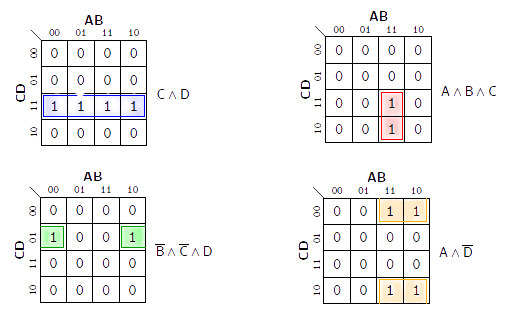
\includegraphics[width=\textwidth]{graphics/karnaugh-veitch-example01}
\end{figure}


\begin{enumerate}
  \item \textbf{Schritt:}
        Finde alle maximalen Zusammenfassungen von Feldern
        
        (dürfen überlappen, aber nicht in größeren Zusammenfassungen vorkommen)
        
        \begin{center}
          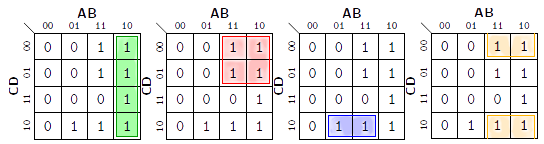
\includegraphics[scale=1]{graphics/karnaugh-veitch-step_01}
        \end{center}
        
        
  \item \textbf{Schritt:}
        Wähle möglichst wenige Zusammenfassungen, die alle Einsen abdecken
        
        \begin{center}
          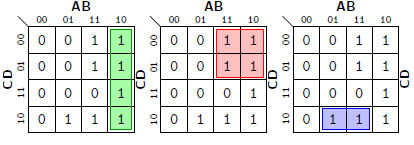
\includegraphics[scale=1]{graphics/karnaugh-veitch-step_02}
        \end{center}
        
        
  \item \textbf{Schritt:}
        Sammle die benötigten Ausdrücke:
        \begin{multicols}{2}
          \begin{align*}
            0 & = \color{red}{(A \wedge \overline{C})}              \\
              & \vee \color{green}{(A \wedge B)}                    \\
              & \vee \color{blue}{(B \wedge C \wedge \overline{D})}
          \end{align*}
          \columnbreak
          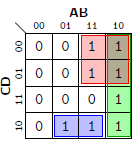
\includegraphics[scale=1]{graphics/karnaugh-veitch-step_03}
        \end{multicols}
\end{enumerate}

\begin{infobox}
  Natürlich kann die Minimierung nicht nur durch Zusammenfassen von Einsen, sondern, 
  unter Rückgriff auf die Dualität der Booleschen Gesetze bzw. 
  die Dualität der disjunktiven und der konjunktiven Normalform, 
  auch durch Zusammenfassen von Nullen durchgeführt werden.
  
  Da das Ergebnis eine Konjunktion von Disjunktionen ist (analog zur konj. Normalform) 
  müssen die Variablenwerte, 
  die die Zusammenfassungen beschreiben negiert werden
\end{infobox}
\subsubsection{Quine-McCuskey-Algorithmus}
Eine Minimierung logischer Funktionen mit bis zu sechs Argumenten ist zwar mit erweiterten 
Karnaugh-Veitch-Diagrammen im Prinzip möglich, aber unhandlich. Ein besserer Weg besteht 
in der Verwendung eines anderen Verfahrens des \textbf{Quine-McClunskey-Algorithmus}.

\begin{enumerate}
  \item \textbf{Schritt:} Bilde die disjunktive (analog auch konmjunktive) Normalform der zu minimierenden Funktion.
  \item \textbf{Schritt:} Finden der \textbf{Primimplikanten}.
        \begin{itemize}
          \item Vereinige Terme, in denen eine einzelne Variable
                in dem einen Term als positives, im anderen als negatives Literal auftritt.
                (Der gleiche Term darf für mehrere Vereinigungen verwendet werden.)
                
                \begin{align*}
                  (A_1 ... A_i ... A_n) \vee (A_1 ... \overline{A_i} ... A_n)
                   & = A_1 ... A_{i-1} A_{i+1} ... A_n \wedge (A_i \vee \overline{A_i})  \\
                   & = A_1 ... A_{i-1} A_{i+1} ... A_n \wedge 1                          \\
                   & = A_1 ... A_{i-1} A_{i+1} ... A_n                                  
                \end{align*}
          \item Wiederhole dies Rekursiv mit den Vereinigungsergebnissen, bis keine weiteren Vereinigungen mehr möglich sind.
          \item Vernachlässige alle Terme, die mit anderen Vereinigt wurden.
          \item Übrig bleiben die sogenannten \textbf{Primimplikanten}
        \end{itemize}
        
        \begin{center}
          \includegraphics[width=\textwidth]{graphics/Quine–McCluskeyAlgorithmus_step_01.png}
        \end{center}
        
  \item \textbf{Schritt:} Aufstellen und Auswerten der Primimplikantentabelle
        \begin{itemize}
          \item Spalten: Minterme, Zeilen: Primimplikanten
          \item Finde wesentliche Primimplikanten (aufsuchen der Spalten mit nur einer Markierung)
                
                Eine systematische Methode für diese Auswahl von Primimplikanten ist \textbf{Petricks Algorithmus}
        \end{itemize}
        \begin{center}
          \includegraphics[scale=1]{graphics/Quine–McCluskeyAlgorithmus_step_02.png}
        \end{center}
        
        \begin{itemize}
          \item[\color{red} $\bullet$ ] Abdeckung nur durch einen Primimplikanten $\rightarrow$ wesentlich
          \item[\color{blue} $\bullet$ ] Abdeckung auch durch wesentliche Primimplikanten.
          \item[\color{gray} $\bullet$ ] Nicht benötigte Abdeckungen
        \end{itemize}
\end{enumerate}


\begin{infobox}
  Primimplikanten des Quine-McCluskey-Algorithmus entsprechen 
  Feld-Zusammenfassungen in Karnaugh-Veitch-Diagrammen.
  
  Dementsprechend gibt es auch wesentliche Zusammenfassungen in Karnaugh-Veitch-Diagrammen. 
  (Feldergruppen, die von keiner der anderen Gruppen abgedeckt werden)
\end{infobox}
\begin{figure}[h]
  \begin{minipage}{0.6\textwidth}
    \begin{itemize}
      \item[\color{green} Grün] entspricht dem 4er Primimplikanten 10--
      \item[\color{red} Rot\ ] entspricht dem 4er Primimplikanten -110
      \item[\color{blue} Blau] entspricht dem 2er Primimplikanten -110
      \item[\color{yellow} Gelb] entspricht dem 4er Primimplikanten 1--0
    \end{itemize}
  \end{minipage}
  \hfill
  \begin{minipage}{0.4\textwidth}
    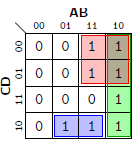
\includegraphics{graphics/karnaugh-veitch-step_03.png}
  \end{minipage}
\end{figure}
%TODO: 02 Schaltungstechnik p29

\subsection{Petricks Algorithmus}
Nicht immer decken die wesentlichen Primimplikanten alle Minterme ab. 
In diesem Fall müssen aus den restlichen Primimplikanten geeignete ausgewählt werden, 
um die verbleibenden Minterme abzudecken.


\begin{enumerate}
  \item \textbf{Schritt:} Bilde eine reduzierte Primimplikantentabelle
        
        Diese enthält nur noch die noch nicht abgedeckten Minterme und die nicht wesentlichen Primimplikanten.
        
  \item \textbf{Schritt:} Ordne jedem Primimplikanten eine Auswahlvariable $P_i$ zu.
        
  \item \textbf{Schritt:} Bilde für jeden Minterm (Spalte) die Disjunktion der Auswahlvariablen.
        
        Alle Primimplikanten, die diesen Minterm abdecken werden mit einer Disjunktion verknüpft.
        
  \item \textbf{Schritt:} Verknüpfe alle Disjunktionen zu einer Konjunktion $C$.
        
  \item \textbf{Schritt:} Wandle Konjunktion $C$ durch die Distributivgesetze in eine Disjunktion $D'$ um
        
        Nun ergibt sich eine Disjunktion aus Konjunktionen, die jeweils alle Minterme abdecken.
        $$(P_1 \wedge P_2 \wedge P_3) \vee (P_2 \wedge P_3 \wedge P_4) \vee (P_3 \wedge P_5)$$
        
  \item \textbf{Schritt:} Wähle die Konjunktionen aus $D'$, mit den wenigsten Primimplikanten
        
        $P_3 \wedge P_5$
        
\end{enumerate}

\begin{figure}[H]
  \begin{minipage}{0.6\textwidth}
    \begin{table}[H]
      \centering
      \begin{tabular}{|cc|cccccl|}
        \hline
                                              &     & \multicolumn{6}{c|}{Minterme (Konjunktionen)}                                                                                                                              \\ \hline
        \multicolumn{2}{|c|}{Primimplikanten} & 000 & 001                                           & 010                    & 101                    & 110                    & 111                                             \\ \hline
        \multicolumn{1}{|c|}{$P_1$}           & 00- & \color{blue} $\bullet$                        & \color{blue} $\bullet$ &                        &                        &                        &                        \\
        \multicolumn{1}{|c|}{$P_2$}           & 0-0 & \color{blue} $\bullet$                        &                        & \color{blue} $\bullet$ &                        &                        &                        \\
        \multicolumn{1}{|c|}{$P_3$}           & -01 &                                               & \color{blue} $\bullet$ &                        & \color{blue} $\bullet$ &                        &                        \\
        \multicolumn{1}{|c|}{$P_4$}           & -10 &                                               &                        & \color{blue} $\bullet$ &                        & \color{blue} $\bullet$ &                        \\
        \multicolumn{1}{|c|}{$P_5$}           & 1-1 &                                               &                        &                        & \color{blue} $\bullet$ &                        & \color{blue} $\bullet$ \\
        \multicolumn{1}{|c|}{$P_6$}           & 11- &                                               &                        &                        &                        & \color{blue} $\bullet$ & \color{blue} $\bullet$ \\ \hline
      \end{tabular}
    \end{table}
  \end{minipage}
  \begin{minipage}{0.4\textwidth}
    \begin{align*}
             & (P_1 \vee P_2)\ (001)   \\
      \wedge & (P_1 \vee P_3)\ (001) & \\
      \wedge & (P_2 \vee P_4)\ (010) & \\
      \wedge & (P_3 \vee P_5)\ (101) & \\
      \wedge & (P_4 \vee P_6)\ (110) & \\
      \wedge & (P_5 \vee P_6)\ (111) & \\
    \end{align*}
  \end{minipage}
\end{figure}


\section{Programmierbare Logikarrays}
Alle betrachteten Minimierungsergebnisse haben die folgende allgemeine Form:
$$o = (i_1 \wedge \overline{i_2} \wedge \overline{i_3} \wedge ...) \vee (\overline{i_1} \wedge i_2 \wedge \overline{i_3} \wedge ...) \vee (\overline{i_1} \wedge \overline{i_2} \wedge i_3 \wedge ...) \vee ... $$
Alle Boolesche Formeln können in diese Form gebracht werden, denn es handelt sich um eine Disjunktion von Konjunktionen von Literalen (sum of products, SOP)

\begin{defbox} [Programmierbare Logikarrays]
  Programmierbare Logikarrays (programmable logic array, PLAs) sind solche Formeln "realisiert in Hardware".
  \begin{itemize}
    \item Alle Eingaben $i_k$ und ihre Negation $\overline{i_k}$ sind verfügbar
    \item Die Eingaben werden über AND-Gatter verknüpft
    \item Die Ausgaben der AND-Gatter werden durch OR-Gatter verknüpft
    \item Ein PLA wird durch Entfernen von Verbindungen "konfiguriert" ("programmiert")
  \end{itemize}
\end{defbox}

\subsubsection{Gatterimplementierung von Originalfunktion und disjunkt. Normalform}

\begin{figure}[H]
  \begin{minipage}[t]{0.4\textwidth}
    \caption{Mehr Gatter, aber standardisierte Struktur}
    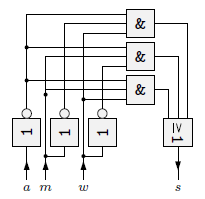
\includegraphics[width=\textwidth]{graphics/PLA_example_normal.png}
  \end{minipage}
  \hfill
  \begin{minipage}[t]{0.4\textwidth}
    \caption{Weniger Gatter, aber Struktur abhängig von jeweiliger Funktion}
    \centering
    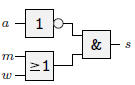
\includegraphics[width=\textwidth]{graphics/PLA_example_original.png}
  \end{minipage}
\end{figure}



\subsection{Allgemeine Struktur}
Jede Funktion in disjunktiver Normalform kann durch eine Standard-Gatterstruktur dargestellt werden:
\begin{itemize}
  \item Einem NOT-Gatter (Inverter), sodass für jede Eingabe negiert und unnegiert zur verfügung steht.
  \item Einem AND-Array, zur Berechnung der Konjunktionen
  \item Einem OR-Array, zur disjunktiven Verknüpfung der Konjunktionen
\end{itemize}


\subsection{Hardware-Implementation}

\begin{figure}[h]
  \begin{minipage}[t]{0.45\textwidth}
    \caption{Originale Darstellung von Schaltungen}
    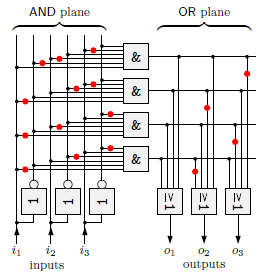
\includegraphics[height=\textwidth]{graphics/PLA_implementation.png}
    Bei Auslieferung sind Logikarrays komplett verbunden (an jedem UND-Gatter liegen alle negierte und unnegierte Eingaben an).
    Beim "programmieren" des Logikarrays werden die rot markierten Verbindungen getrennt
  \end{minipage}
  \hfill
  \begin{minipage}[t]{0.45\textwidth}
    \caption{Vereinfachte Darstellung von Schaltungen}
    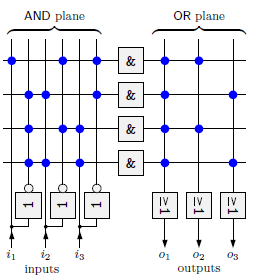
\includegraphics[height=\textwidth]{graphics/PLA_implementation_simplification.png}
    Zur Vereinfachung stellt man nur eine Linie je Gatter dar und markiert die \textbf{Verbindungen}
  \end{minipage}
\end{figure}

Für eine elektronische Implementierung (durch Transistoren) sind AND- und OR-Gatter nicht besonders gut geeignet.
Besser geeignet sind NAND- und NOR-Gatter (und ggf. NOT-Gatter).


\section{Hardware-Beschreibungssprache}
\begin{defbox}[Hardware-Beschreibungssprache]
  Eine formale Sprache, mit der Operationen von integrierten Schaltungen und ihr Design beschrieben sowie in Simulationen getestet werden können.
  \begin{itemize}
    \item Spezifieren von dem Verhalten von Bausteinen (Schnittstelle), sowie Implementierung aus Elementargattern.
    \item Simulator kann Elementargatter (und damit inderekt alle aus diesen zusammengesetzten Bausteine) simulieren
    \item Simuliertes Verhalten kann automatisch mit Schnittstelle verglichen werden (\textit{automatische Fehlerüberprüfung})
  \end{itemize}
\end{defbox}

\subsection{Aufbau}
Hardware-Beschreibung eines Bauteils durch drei Dateien:
\begin{itemize}
  \item $*.cmp$ Beschreibung der Schnittstelle durch Ein-/Ausgabetupel
  \item $*.hdl$ Beschreibung der Implementierung durch Gatterzusammenschaltung
  \item $.tst$ Befehle zum Durchführen eines Funktionstests
\end{itemize}

% And.cmp
% a b out
% 0 0 0
% 0 1 0
% 1 0 0
% 1 1 1

% And.hdl
% CHIP And
% { IN a, b;
% OUT out;
% IN a, b;
% OUT out;
% PARTS:
% Nand(a = a, b = b, out = x);
% Not(in = x, out = out);
% }

% load And.hdl,
% output-file And.out,
% compare-to And.cmp,
% output-list a b out;
% set a 0, set b 0, eval, output;
% set a 0, set b 1, eval, output;
% set a 1, set b 0, eval, output;
% set a 1, set b 1, eval, output;

LESEN:\\
The Elements of Computing Systems: Building a Modern Computer from First Principles\\
Noam Nisan \& Shimon Schocken\\
MIT Press, Cambridge, MA, USA 2008\\
Bearbeiten: http://www1.idc.ac.il/tecs/projects/01/index.htm
66\\

\chapter{Binärarithmetik \& Ihre Implementierung}
\section{Erinnerung: Arithmetik}
\subsection{Zahlensysteme}
Im prinzip kann jede beliebige Zahl als Basis eines Zahlensystems gewählt werden.
Das in der Rechnertechnik verwendete \textit{Binärsystem} (Basis 2) hat den Vorteil der kleinstmöglichen Zahl an Ziffernzeichen, nämlich nur zwei:
$$0,\ 1$$
Das auch häufig verwendete \textit{Hexadezimalsystem} (Basis 16):
$$0,\ 1,\ 2,\ 3,\ 4,\ 5,\ 6,\ 7,\ 8,\ 9,\ A,\ B,\ C,\ D,\ E,\ F$$

\subsection{Addition und Subtraktion}

\begin{figure}[H]
  \begin{minipage}[T]{.45\textwidth}
    Addition und Subtraktion kann sehr leicht stellenweise in einem Stellensystem ausgeführt werden.
    
    Einziges Problem ist die Behandlung von \textit{Stellenüberlauf} und \textit{Stellenunterlauf}. 
    In diesen Fällen entsteht ein \textit{Übertrag}.
    
    Diese Rechenschemata sind nicht nur im Dezimalsystem, sondern im Prinzip in jedem Zahlensystem anwendbar.
    
  \end{minipage}
  \begin{minipage}[T]{.45\textwidth}
    \centering
    \begin{tabular}{LLLLLLLLL}
        & 4      & 6 & 7      & 8 & 5 & 3      & 9      & 9 \\
      + & 2\cred & 8 & 0\cred & 7 & 1 & 2\cred & 3\cred & 4 \\ \hline
      = & 7      & 4 & 8      & 5 & 6 & 6      & 3      & 3
    \end{tabular}
    \begin{tabular}{LLLLLLLLL}
        & 4      & 6 & 7      & 8 & 5 & 3      & 9      & 9 \\
      - & 2\cred & 8 & 0\cred & 7 & 1 & 2\cred & 3\cred & 4 \\ \hline
      = & 4      & 6 & 7      & 8 & 5 & 3      & 9      & 9
    \end{tabular}
  \end{minipage}
\end{figure}


\subsection{Multiplikation und Division}
\begin{figure}[H]
  \begin{minipage}[T]{.4\textwidth}
    
    Die Multiplikation wird auf eine Summe von Stellenprodukten zurückgeführt.    
    
    Hierin besteht das Hauptproblem darin, den richtigen Stellenfaktor zu bestimmen. 
    
    Meist wird er geschätzt, anschließend ausprobiert und gegebenenfalls die Schätzung korrigiert.
  \end{minipage}
  \hfill
  \begin{minipage}[T]{.55\textwidth}
    \caption{Beispiel von Multiplikation}
    \centering
    \begin{tabular}{LLLLLLLLLLLLLL|L}
             &   &   &   &   &   & 4 & 6 & 7 & 8 & 5 & 3 & 9 & 9 &   \\
      \times &   &   &   &   &   &   &   &   & 9 & 6 & 4 & 3 & 1 &   \\ \hline 
             &   &   &   &   &   & 4 & 6 & 7 & 8 & 5 & 3 & 9 & 9 & 1 \\
      +      &   &   &   & 1 & 4 & 0 & 3 & 5 & 6 & 1 & 9 & 7 &   & 3 \\
      +      &   &   & 1 & 8 & 7 & 1 & 4 & 1 & 5 & 9 & 6 &   &   & 4 \\
      +      &   & 2 & 8 & 0 & 7 & 1 & 2 & 3 & 9 & 4 &   &   &   & 6 \\
      +      & 4 & 2 & 1 & 0 & 6 & 8 & 4 & 9 & 1 &   &   &   &   & 9 \\ \hline
      =      & 4 & 5 & 1 & 1 & 5 & 6 & 2 & 8 & 1 & 0 & 9 & 6 & 9 & 
    \end{tabular}
  \end{minipage}
  % TODO: Evtl noch Division? 03 p13
\end{figure}


\section{Binäre Arithmetik und Implementierung durch Schaltkreise}
Die beiden Ziffern des Binärsystems können direkt durch Schalter Implementiert werden 
($0$: offen (falsch), $1$: geschlossen (wahr))

\section{Addition}
Die Addition ist die einfachste und am häufigsten verwendete Operation in der arithmetisch-logischen Einheit,
da sie sich direkt in Wahrheitstafeln übersetzen lassen:

\begin{figure}[H]
  \begin{minipage}[T]{.7\textwidth}
    An der Addition von zwei Bits mit Wert $1$ zeigt, 
    
    warum wir für den Ein-Bit-Addierer zwei Ausgänge benötigen:
    \begin{itemize}
      \item Die \textit{Summe} (sum, s)
      \item Den \textit{Übertrag} (carry, c)
    \end{itemize}
    Die bitweise Addition kann offenbar auch durch (Logik-)gatter implementiert werden.
  \end{minipage}
  \hfill
  \begin{minipage}[T]{.2\textwidth}
    \begin{tabular}{|LL|LL|}
      \hline
      x & y & s & c \\ \hline
      0 & 0 & 0 & 0 \\ \hline
      1 & 0 & 1 & 0 \\ \hline
      0 & 1 & 1 & 0 \\ \hline
      1 & 1 & 0 & 1 \\ \hline
    \end{tabular}
  \end{minipage}
  \hfill
\end{figure}


\subsection{Halbaddierer}
\begin{figure}[H]
  \begin{minipage}[T]{.45\textwidth}
    Wegen der möglichkeit eines Übertrags benötigt man für die Addition nicht nur eine Boolesche Funktion, 
    sondern zwei (wobei die zweite den Übetrag bestimmt)
    
    \begin{center}
      $c = x \wedge y$ $s = (x \wedge \overline{y}) \vee (y \wedge \overline{x})$
    \end{center}
  \end{minipage}
  \hfill
  \begin{minipage}[T]{.45\textwidth}
    \caption{Halbaddierer}
    \centering
    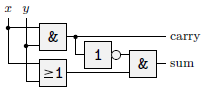
\includegraphics{graphics/halbaddierer_01}
  \end{minipage}
\end{figure}

\begin{figure}[H]
  \begin{minipage}[T]{.45\textwidth}
    Verknüpfung der beiden Funktionen erlaubt eine Implementierung mit weniger Gattern:
    $$s = (x \wedge \overline{(x \wedge y)} \vee (y \wedge \overline{(x \wedge y)}))$$
    \begin{center}
      \small (Ableitbar über Axiome)
    \end{center}
  \end{minipage}
  \hfill
  \begin{minipage}[T]{.45\textwidth}
    \caption{Halbaddierer mit weniger Gattern}
    \centering
    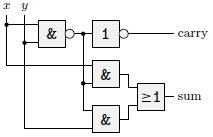
\includegraphics{graphics/halbaddierer_02}
  \end{minipage}
\end{figure}

\begin{figure}[H]
  \begin{minipage}[T]{.45\textwidth}
    Durch weiteres Ausnutzen der Booleschen Gesetze zur Vereinfachung und
    durch Nutzung anderer, zusammengesetzter Gatter ergibt sich dann eine deutlich kleinere Schaltung:
    \begin{align*}
      \centering
      s 
       & = (x \wedge \overline{y}) \vee (\overline{x} \wedge y) \\
       & = x \oplus y                                           \\
    \end{align*}
  \end{minipage}
  \hfill
  \begin{minipage}[T]{.45\textwidth}
    \caption{Optimierter Halbaddierer}
    \centering
    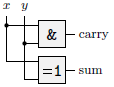
\includegraphics[scale=1.3]{graphics/halbaddierer_optimiert}
  \end{minipage}
\end{figure}


\subsection{Volladdierer}
\begin{figure}[H]
  \begin{minipage}[t]{.45\textwidth}
    Um Addition nicht nur für ein Bit, sondern für $n$ Bits, $n\geq2$, zu implementieren,
    braucht man einen
    
    \par \textit{Addierer mit drei Eingängen}:
    
    Ein Volladdierer berücksichtigt den Übertrag einer vorangehenden Addition
  \end{minipage}
  \hfill
  \begin{minipage}[t]{.45\textwidth}
    \centering
    \begin{tabular}[t]{|LLL|LL|}
      \hline
      x & y & c_{in} & s & c_{out} \\ \hline
      0 & 0 & 0      & 0 & 0       \\
      1 & 0 & 0      & 1 & 0       \\
      0 & 1 & 0      & 1 & 0       \\
      1 & 1 & 0      & 0 & 1       \\
      0 & 0 & 1      & 1 & 0       \\
      1 & 0 & 1      & 0 & 1       \\
      0 & 1 & 1      & 0 & 1       \\
      1 & 1 & 1      & 1 & 1       \\ \hline 
    \end{tabular}
    
  \end{minipage}
\end{figure}

\begin{figure}[H]
  \begin{minipage}[t]{.45\textwidth}
    Ein Volladdierer berechnet die Funktion
    $$s = (x + y) +x_{in}$$
    Aus diesem Grund wird er am einfachsten aus zwei Halbaddierern zusammengesetzt (mit $z = x_{in}$)
  \end{minipage}
  \hfill
  \begin{minipage}[t]{.45\textwidth}
    \centering
    \vspace{0pt}
    \caption{Volladdierer}
    \centering
    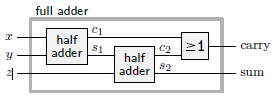
\includegraphics{graphics/volladdierer}
  \end{minipage}
\end{figure}

\subsection{$n$-Bit-Addierer}
\subsubsection{$n$-Bit-Übertragungskette-Addierer}
\begin{defbox}[Übertragungskette-Addierer]
  In einem $n$-Bit-Übertragungskette-Addierer wird mithilfe von $n$ Volladdierern Addition durchgeführt
\end{defbox}
\begin{figure}[H]
  \begin{minipage}[t]{.45\textwidth}
    ein $n$-Bit-Übertr.kette-Addierer (carry ripple adder) für $C = A + B$
    kann leicht aus $n$ Volladdierern zusammengesetzt werden\\
    \par \textit{Probleme}:
    \begin{itemize}
      \item Übertrag breitet sich wellenartig durch die Addiererkette aus
      \item Volladdierer $add_k$ kann erst anfangen, wenn $add_{k-1}$ seine Berechnung abgeschlossen hat
    \end{itemize}
  \end{minipage}
  \hfill
  \begin{minipage}[t]{.45\textwidth}
    \caption{Übertragzungskette-Addierer}
    \centering
    \vspace{0pt}
    \includegraphics[width=\textwidth]{graphics/n-bit-addierer_übertragungskette}
  \end{minipage}
\end{figure}

\subsubsection{$n$-Bit-Übertragsauswahl-Addierer}
\begin{defbox}[Übertragsauswahl-Addierer]
  In einem $n$-Bit-Übertragsauswahl-Addierer werden die Summen des unteren Halbwortes (Bits 0 bis $\frac{n}{2}-1$) und 
  des oberen Halbwortes (Bits $\frac{n}{2}-1$ bis $n$) parallel berechnet.
  
  Dadurch umgeht man die Problematik des wellenartigen Übertrags.
\end{defbox}

\begin{figure}[H]
  \begin{minipage}[t]{.45\textwidth}
    Da der Wert des Übertrags aus dem unteren Halbwort noch nicht bekannt ist, wenn die Summenbildung für das obere
    Halbwort beginnt, wird diese Summe zweimal, in getrennten Schaltungen berechnet:
    \begin{itemize}
      \item Schaltung 1: $c_{in} = 0$
      \item Schaltung 2: $c_{in} = 1$
    \end{itemize}
    \par Wenn der Übertrag des unteren Halbworts berechnet ist, wird er über einen 
    Multiplexer zur Auswahl des richtigen oberen Halbworts benutzt
  \end{minipage}
  \hfill
  \begin{minipage}[t]{.45\textwidth}
    \caption{Übertragungsauswahl-Addierer}
    \centering
    \includegraphics[width=\textwidth]{graphics/n-bit-addierer_übertragungsauswahl}
  \end{minipage}
\end{figure}

\begin{infobox}
  Bei längeren Binärzahlen wird das Prinzip des Übertragungsauswahl-Addierers rekusiv angewandt (d.h., die Halbwörter werden ihrerseits zerlegt)
\end{infobox}

\subsection{Darstellung negativer Zahlen}
\begin{figure}[H]
  \begin{minipage}[t]{.3\textwidth}
    \centering
    \paragraph{Betrag \& Vorzeichen}
    \small Höchstwertiges Bit gibt Vorzeichen an
    
    \underline{Problem}: Zahlen sollten gleiche Stellenzahl aufweisen
  \end{minipage}
  \hfill
  \begin{minipage}[t]{.3\textwidth}
    \centering
    \paragraph{Einerkomplement}
    \small Negation durch Inversion der Zahl
    
    \underline{Problem}: Übertrag, Zwei Darstellungen für Null
  \end{minipage}
  \hfill
  \begin{minipage}[t]{.3\textwidth}
    \centering
    \paragraph{Zweierkomplement}
    \small Negation durch Inversion und Addition von 1
    
    \underline{Problem}: Übertrag, Zwei Darstellungen für Null
  \end{minipage}
\end{figure}

\subsubsection{n-Bit-Addierer \& -Subtrahierer im Zweierkomplement}
\begin{defbox}[Addierer \& Subtrahierer im 2er-Komplement]
  $n$-Bit-Subtrahierer bestehen aus eine, $n$-Bit-Addierer und Gattern, 
  die die Negationsregel implementieren.
  
  \center{Idee: $A-B=A+(-B)$}
\end{defbox}

\begin{figure}[h]
  \caption{Beispiel eines n-Bit-Subtrahierers}
  \centering
  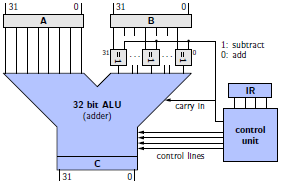
\includegraphics{graphics/n-bit-subtrahierer.png}
\end{figure}

\section{Multiplikation}
%TODO
Binärarithmetik p37ff
\subsection{Multiplikation mit Potenzen der Basis}
\subsection{Multiplikation mit Zweierpotenzen: Bit-Schieben}
\subsection{Allgemeine Binäre Multiplikation}
\subsection{Negative Zahlen}
\subsection{Standardalgorithmusa}
\subsection{Booths Algorithmus}


\section{Die Arithmetisch-Logische-Einheit (Arithmetic Logical Unit. ALU)}
\subsection{Die ALU in der Hack-Architektur}
\subsection{Einbindung der ALU in den Prozessor der Hack-Architektur}


\chapter{Sequentielle Logik}
\section{Sequentielle Logik}
\subsection{Logikschaltungen: Kombinatorische \& Sequentielle Logik}
\begin{figure}[H]
  \begin{minipage}[t]{0.48\textwidth}
    \paragraph{Kombinatorische Logik}
    
    \centering
    
    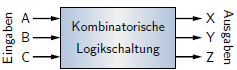
\includegraphics[width=\textwidth]{graphics/kombinatorische_logik}
    
  \end{minipage}
  \hfill
  \begin{minipage}[t]{0.48\textwidth}
    \paragraph{Sequentielle Logik}
    
    \centering
    
    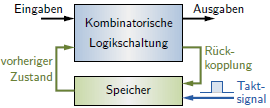
\includegraphics[width=\textwidth]{graphics/sequentielle_logik}
  \end{minipage}
\end{figure}

\begin{figure}[H]
  \begin{minipage}[t]{0.48\textwidth}
    \centering
    \underline{Implementierung: Schaltnetze}
    
    \begin{itemize}
      \item Einfaches Berechnen von Ein- \& Ausgaben
      \item Keine Informationsspeicherung
      \item Zustandslosigkeit
      \item verzögerungsfreie Berechnung
    \end{itemize}
  \end{minipage}
  \hfill
  \begin{minipage}[t]{0.48\textwidth}
    \centering
    \underline{Implementierung: Schaltwerke}
    
    \begin{itemize}
      \item Rückkopplung von Ausgaben auf Eingaben
      \item Explizite Informationsspeicherung
      \item Unterscheidung von Zuständen
      \item Gatterlaufzeiten explizit berücksichtigt
    \end{itemize}
    
  \end{minipage}
\end{figure}

\begin{figure}[H]
  \begin{minipage}[T]{0.45\textwidth}
    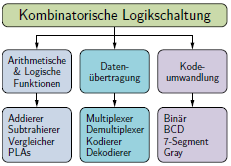
\includegraphics[width=\textwidth]{graphics/kombinatorische_logikschaltung}
  \end{minipage}
  \hfill
  \begin{minipage}[T]{0.45\textwidth}
    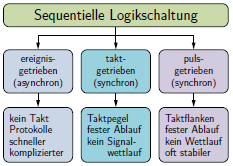
\includegraphics[width=\textwidth]{graphics/sequentielle_logikschaltung}
  \end{minipage}
\end{figure}

\subsection{Prinzip der Rückkopplung}
\begin{defbox}[Rückkopplung]
  \begin{figure}[H]
    \begin{minipage}[T]{0.7\textwidth}
      Durch Rückkopplung werden Ausgaben als Eingabesignal verwendet. 
      Hierdurch kann ein (Ausgabe-) Zustand festgehalten werden, 
      bis ein Ergeignis ihn wieder ändert.
    \end{minipage}
    \hfill
    \begin{minipage}[T]{0.25\textwidth}
      \includegraphics{graphics/rückgekoppelter_2_wege_multiplexer}
    \end{minipage}
  \end{figure}
\end{defbox}

\paragraph{Probleme der Rückkopplung}

Durch Rückkopplung kann es zu (unerwünschten) \textit{Schwingungen} kommen. 
Diese sind ein Beispiel für \textit{Signallaufzeitprobleme}, die durch Rückkopplungen auftreten können).

Ein weiteres Beispiel sind sogenannte \textit{Wettlaufsituationen (Race Conditions)}, die auftreten, 
wenn sich zwei Signale auf zwei oder mehr Wegen ausbreiten, und die Ausgabe davon abhängen kann, 
welches Signal schneller weitergegeben wird

Rückkopplungen lassen sich am leichtesten durch ein zentral erzeugtes \underline{\textit{Taktsignal}} vermeiden, 
das bestimmt, wann Eingaben übernommen werden.

\subsection{Asynchrone und synchrone Schaltwerke}

\begin{figure}[H]
  \begin{minipage}[T]{0.45\textwidth} w
    \centering
    \paragraph{Asynchrone Schaltwerke}
    \begin{itemize}
      \item Direkte Steuerung durch Änderung der Eingangssignale
      \item Wann und ob ein stabiler Zustand erreicht wird von Gatterlaufzeit abhängig
      \item Oft komplizierter, aufwendiger Entwurf
      \item Sehr schnelle Schaltwerke möglich
    \end{itemize}
  \end{minipage}
  \hfill
  \begin{minipage}[T]{0.45\textwidth}
    \centering
    \paragraph{Synchrone Schaltwerke}
    \begin{itemize}
      \item Steuerung durch Taktsignal
      \item Eingangssignale nur zu von Takt festgelegten Zeitpunkten übernommen
      \item Meist einfacher, systematischer Entwurf.
      \item Langsamstes Bauteil bestimmt maximal mögliche Taktfrequenz
    \end{itemize}
  \end{minipage}
\end{figure}

\subsection{Taktsignal (Clock Signal)}

\section{Bistabile Kippstufen}

\section{Register, Zähler und Speicher}

\section{Hardware-Simulation der sequentiellen Logik}




\end{document}


